% =============================================================================
% FILE NAME : 01_fundamentals.tex
% DEPARTMENT: University of Tuebingen
% AUTOR     : Paul Palomero Bernardo & Konstantin Lübeck
% =============================================================================
% CONTENT   : Include for chapter "Fundamentals"
% =============================================================================

Ziel dieses Kapitels ist eine Einführung in die Thematik BlaBlaBla ...

\section{RISC-V}

RISC-V \cite{riscv} is an open standard Instruction Set Architecture (ISA).
RISC-V International is the non profit that provides the open, royalty-free ISA that is RISC-V.
\\\\
RISC-V was originally developed to support computer architecture research and education, but the authors now
aim for RISC-V to also be used in industry implementations \cite{riscv_spec}.

\section{Embedded AI}

With artificial intelligence (AI) becoming more and more contemporary and wide-ranging it is only consequential that is has found its way into embedded devices.
Especially with the \todo{needs proof/citation} rising trend of IoT devices and smart homes
embedded AI has found its way into the hand of consumer homes.
From voice assistants like Amazon's Alexa \cite{alexa} over autonomous robots like the Roomba \cite{roomba} from iRobot to self driving cars like Tesla's autopilot \cite{autopilot} .
However size and power requirements of those devices severely limit their capabilities, which is why the development of specialized hardware to improve performance
and power usage becomes a necessity.\\
% https://ieeexplore.ieee.org/abstract/document/8318006
In my thesis I'm working with the UltraTrail TC-ResNet AI Accelerator \cite{ultratrail}.
An AI Accelerator is a type of hardware accelerator specialized for artificial intelligence (AI) and machine learning (ML) applications, such as neural networks (NN).
A hardware accelerator is a set of custom made hardware that specializes in carrying out one task only, but doing it really well.
It is created to perform solve one problem faster and/or more efficiently than a generic CPU could with the trade-off that it may not be able to do other things at all.
Examples include, but are not limited to, GPUs or, in this case, AI accelerators.\\\\





\section{Rust}

Rust \cite{rustlang} has been the language of choice for the software running on the Pulpissimo \cite{pulpissimo} that I've written for this thesis.

\subsection{Why Rust?}

While C is the industry standard for writing software for embedded systems, and C++ also being fairly popular, Rust has a couple of
advantages over those languages.\\\\
The biggest downside of C is likely the lack of memory safety, which can not only cause software to be less reliable, but
can also make a system vulnerable to different attacks, such as buffer overflows, reading uninitialized variables or use-after-free, which can compromise cybersecurity \cite{memory_safety}.\\
C++ fixes some of those issues due to the availability of smart pointers, but those are fairly 'modern' C++, thus being only available if compilers support more modern
versions of C++ (with C++ 11 starting to introduce many of concepts).
There is also no guarantee that those features have been used in any given program.
The opposite is more likely actually due to the incorporation of older software (library code written with older C++ versions in mind),
compilers not supporting new versions (especially likely with small vendors that don't have the resources to continuously update compilers for their platform),
or developers not keeping up to date with new language features and therefore not being aware of or able to use them.\\\\
Rust on the other hand can (mostly) give compile time guarantees on the software's safety and reliability.

\subsection{Memory safety and  performance}

\subsubsection{Garbage collection}

Most programming languages that try to achieve memory safety use a garbage collector to do that \cite{java_garbage_collector}.
The downside of a garbage collector however is unpredictable latency (the running program has to be stopped while the garbage collector is running) and a hit in performance.
A garbage collector first identifies pieces of memory that are no longer used \ref{fig:gc_mark}.
Then the marked pieces of memory are periodically deleted \ref{fig:gc_delete}.
After the deletion the garbage collector will 'compact' the memory to avoid memory fragmentation and improve the speed of future allocations.

\begin{figure}[htb]
    \centering
    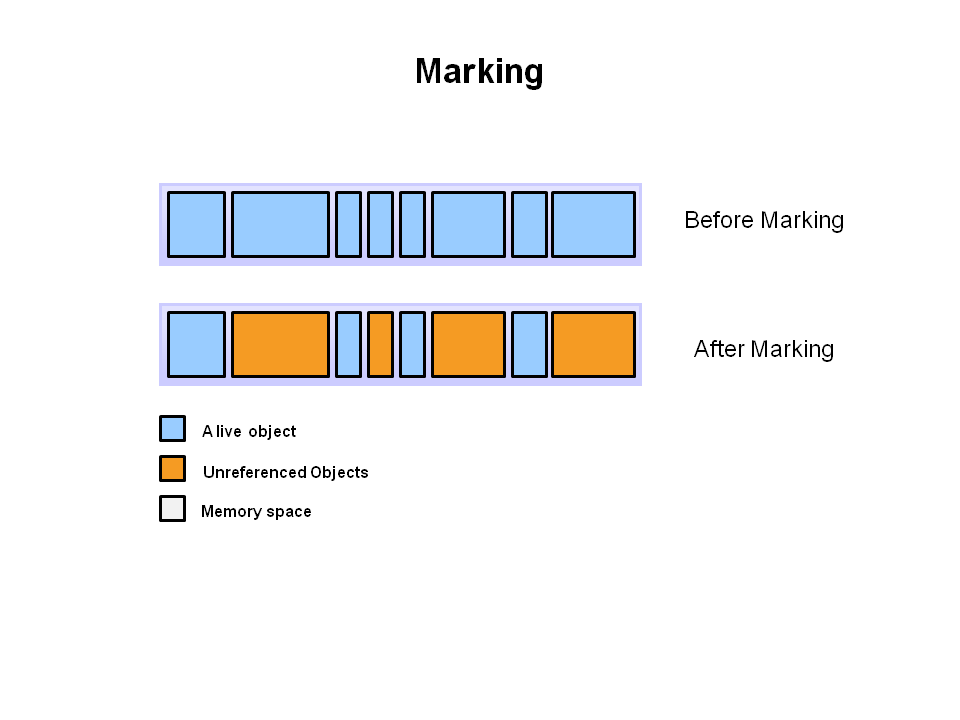
\includegraphics[width=0.9\textwidth]{figures/fundamentals_garbage_collector_marking.PNG}
    \caption[Illustration: Garbage Collector marking memory for deletion\\Source: https://www.oracle.com/webfolder/technetwork/tutorials/obe/java/gc01/images/gcslides/Slide3.png]{Garbage Collector marking memory for deletion}
    \label{fig:gc_mark}
\end{figure}

\begin{figure}[htb]
    \centering
    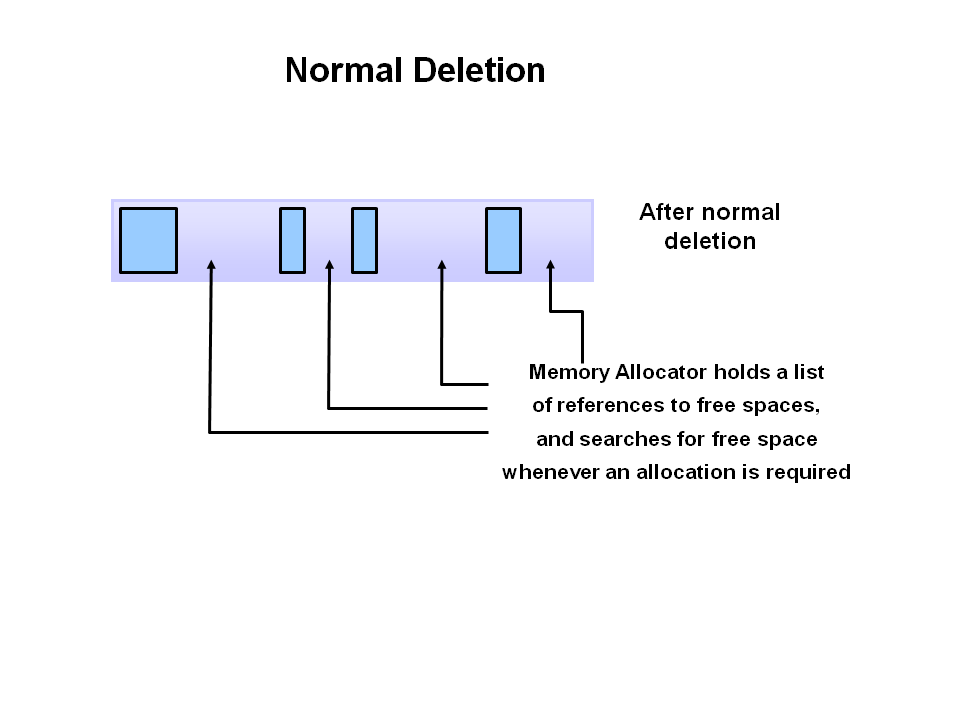
\includegraphics[width=0.9\textwidth]{figures/fundamentals_garbage_collector_deletion.PNG}
    \caption[Illustration: Garbage Collector deleting marked memory\\Source: https://www.oracle.com/webfolder/technetwork/tutorials/obe/java/gc01/images/gcslides/Slide1b.png]{Memory layout after deletion of unused pieces of memory}
    \label{fig:gc_delete}
\end{figure}

\begin{figure}[htb]
    \centering
    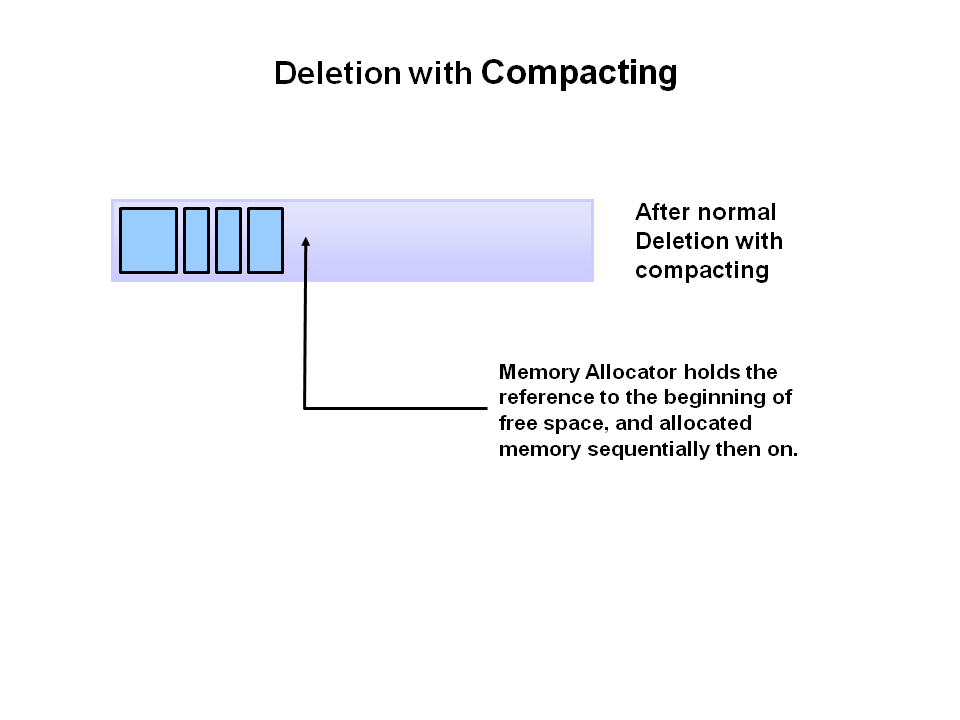
\includegraphics[width=0.9\textwidth]{figures/fundamentals_garbage_collector_compacting.PNG}
    \caption[Illustration: Garbage Collector compacting memory\\Source: https://www.oracle.com/webfolder/technetwork/tutorials/obe/java/gc01/images/gcslides/Slide4.png]{Memory layout after compacting}
    \label{fig:gc_compact}
\end{figure}

\subsubsection{Ownership in Rust}

Rust uses an 'ownership' model \cite{rust_ownership} to make memory safety guarantees at compile time and without the need of a garbage collector,
which is good for safety, and does not negatively impact performance or latency.

% TODO explain ownership

\section{Microphone technology}

A microphone consists of a diaphragm and a transducer.
Sound waves cause the diaphragm to vibrate, and
the transducer turns those vibrations into an electrical signal.

\subsection{I2S}

The inter-IC sound ($I^2S$) \cite{i2s} bus is a serial link that has been developed especially for digital audio.
It uses three lines, one serial data line (SD), one continuous serial clock line (SCK) and one word select line (WS).
$I^2S$ can be used in different configurations, but the master always provides WS and SCK.

\subsubsection{Serial Data}

The data consists of signed integers (in two's complement).
Due to possible differences between the word lengths of transmitter and receiver,
the MSB is transmitted first.

% So neither transmitter nor receiver need any knowledge about the capabilities of the other.
% TODO finish explanation

\subsubsection{Word Select}

Word select determines the transmission channel, where 0 means the left channel and 1 means the right one.
It can be changed on a trailing or leading edge of the clock signal and the WS line changes one clock period
before the MSB is transmitted.
For the purpose of what I do in this thesis, WS is not relevant an will be tied to ground unless mentioned otherwise.

\subsection{Pulse Density Modulation}

Pulse Density Modulation (PDM) is one way to represent an analog signal with a binary signal.
The density of high/low signals at a given sampling rate encodes the state of the analog signal.
So the analog signal is encoded using only 1 bit at a high sampling rate.\\
Therefore a constant bitstream of 1s would represent that the amplitude of the analog signal is maxed out,
while a constant bitstream of 0s would represent that the amplitude of the analog signal is at it's lowest value.
Alternating 1s and 0s represent an amplitude of exactly 0.\\\\
\
\
% TODO explain PDM
\
While many digital audio systems use Pule Code Modulation (PCM), which, in contrast to PDM, uses multiple bits to represent a signal,
PDM is used a lot in mobile phones \cite{pdm_utexas} due to its simplicity and low cost.
However 1bit PCM would be much too noisy to be useful.
So to counteract the noise increase of only using 1 bit the signal is 'oversampled', thereby increasing the bandwidth of the system.
However the new spectrum that is created by oversampling the signal has a frequency that is too high for the human ear.
Now the only thing that is left to do is 'push' the noise into that new spectrum, thus removing it from the audible signal.
This can be done using 'Noise Shaping'.

\subsubsection{Noise Shaping}

Noise Shaping...


